\chapter{Trees reveal the importance of measures in SLZ} \label{ch:bagging}

%--------------------------
\section{Introduction} \label{sec:bagging_intro}
%--------------------------

The MDS analysis presented in Chapter~\ref{ch:acousticlandscape} helps us to understand the acoustic landscape of SLZ. This helps reveal the multidimensional nature of voice quality and how all the acoustic measures work together to produce that acoustic landscape. The chapter also discussed how certain measures contributed more weight than other acoustic measures to each of the different dimensions. However, it does not tell us what measures are more important in separating the voice qualities from from one another. This is where decision trees can be most helpful.

%--------------------------
\section{What are Decision Trees} \label{sec:bagging_what}
%--------------------------

Decision trees are a statistical tool that helps to reveal which variables divide the space under investigation. Essentially, this is done by stratifying or segmenting the predictor space into some number of simpler regions. The rules that divide the space into these regions are based on some aspect of the variables (see \cite{hastieElementsStatisticalLearning2009,jamesIntroductionStatisticalLearning2021} for explanations on the statistics and how to conduct this in R). 

These trees can be used for both regression and classification. In the case of regressions, it splits the predictor space into regions and calculates how the item under discussion behaves in each region. This process of splitting into regions and calculating how something responds in that region continues until some stopping rule is applied, which is usually defined to some number of terminal nodes. This resulting tree is rather large and is then pruned based on the cost-complexity pruning to a subset of itself. This subsetted tree is the tree that has minimized its cost-complexity criterion of all potential subsets. Meaning that it balances the trade-off between the complexity of the tree and its fit to the data. 

In the case of classification, the algorithms that result in a tree are very similar to those used for regression trees. The main difference in algorithm comes from what is used to split the nodes and how the tree is pruned. Additionally, instead of predicting a continuous outcome like with regression trees, classification trees predict a categorical outcome. The predictor space is divided into regions, and within each region, the majority class is assigned as the predicted class for that region. This process continues until a stopping rule is applied, similar to regression trees. The resulting tree can also be pruned to avoid overfitting, using a cost-complexity criterion.

Decision trees are easy to interpret and visualize, making them a popular choice for understanding the structure of the data. However, they are prone to overfitting, especially with small datasets. To remedy this issue techniques such as bagging \citep{breimanBaggingPredictors1996} and random forests \citep{breimanRandomForests2001} were introduced in order to improve the performance and robustness of decision trees. 

%-----------------------------
\section{Decision trees in linguistics}\label{}
%-----------------------------

The use of decision trees in linguistics is not new. One of the first uses was done by \citet{tagliamonteModelsForestsTrees2012}, where they were illustrated the use of decision trees in investigating which sociolinguistic factors were the most important in the use of \textit{was} versus \textit{were} in York English. Recently, decision trees were used to show which acoustic measures were the most important in making the split in the acoustic space for voice quality \citep{keatingCrosslanguageAcousticSpace2023}. 

In their study, \citet{keatingCrosslanguageAcousticSpace2023} performed an simple decision tree analysis to suppliment their MDS analysis of 11 languages and their voice quality contrasts. 

\begin{figure}[!h]
    \centering
    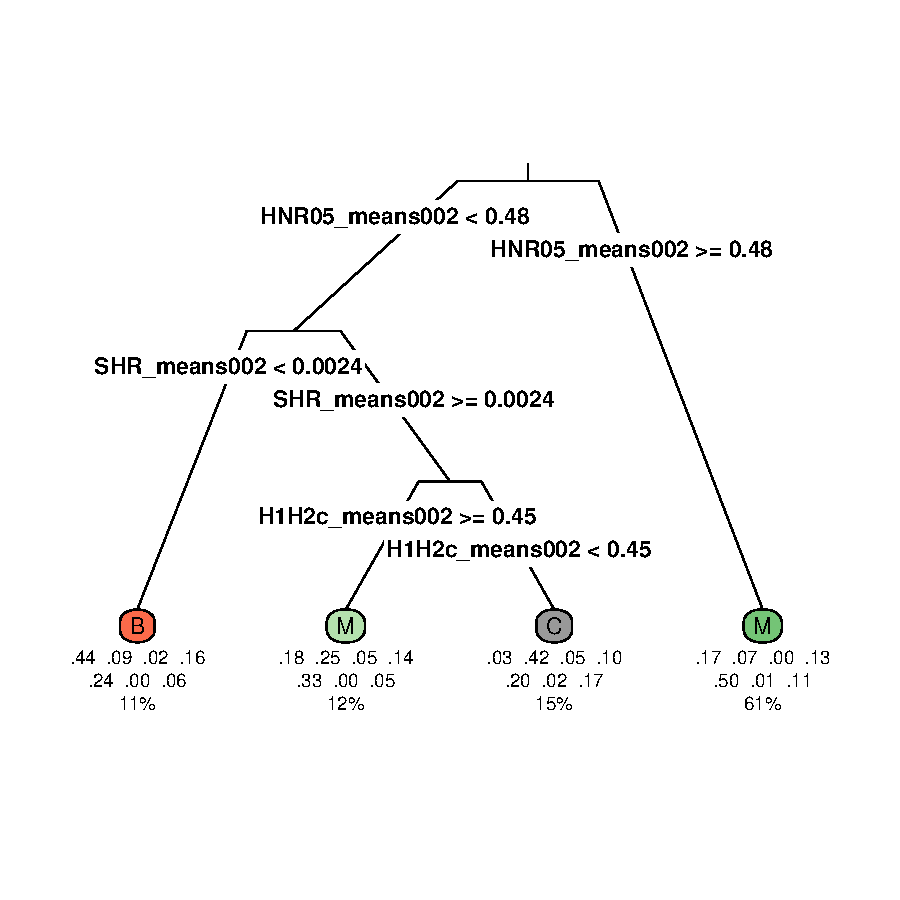
\includegraphics[width = 0.9\linewidth]{images/keating_tree.pdf}
    \caption{Classification tree of phonation categories from \citet{keatingCrosslanguageAcousticSpace2023}. Abbreviations used in this figure are: {HNR05_means002}: harmonics-to-noise ratio over the frequency range from 0 Hz to 500 Hz for the middle third of each vowel; {SHR_means002}: subharmonic-to-harmonic ratio for the middle third of each vowel; {H1H2c_means002}: H1* − H2* for the middle third of each vowel; B: breathy, M: modal, and C: creaky phonation categories.}
    \label{fig:keating_tree}
\end{figure}

In the analysis presented in this chapter, I will make use of bagging trees to assess the importance of the different 
